% Options for packages loaded elsewhere
\PassOptionsToPackage{unicode}{hyperref}
\PassOptionsToPackage{hyphens}{url}
\documentclass[
]{article}
\usepackage{xcolor}
\usepackage[margin=1in]{geometry}
\usepackage{amsmath,amssymb}
\setcounter{secnumdepth}{-\maxdimen} % remove section numbering
\usepackage{iftex}
\ifPDFTeX
  \usepackage[T1]{fontenc}
  \usepackage[utf8]{inputenc}
  \usepackage{textcomp} % provide euro and other symbols
\else % if luatex or xetex
  \usepackage{unicode-math} % this also loads fontspec
  \defaultfontfeatures{Scale=MatchLowercase}
  \defaultfontfeatures[\rmfamily]{Ligatures=TeX,Scale=1}
\fi
\usepackage{lmodern}
\ifPDFTeX\else
  % xetex/luatex font selection
\fi
% Use upquote if available, for straight quotes in verbatim environments
\IfFileExists{upquote.sty}{\usepackage{upquote}}{}
\IfFileExists{microtype.sty}{% use microtype if available
  \usepackage[]{microtype}
  \UseMicrotypeSet[protrusion]{basicmath} % disable protrusion for tt fonts
}{}
\makeatletter
\@ifundefined{KOMAClassName}{% if non-KOMA class
  \IfFileExists{parskip.sty}{%
    \usepackage{parskip}
  }{% else
    \setlength{\parindent}{0pt}
    \setlength{\parskip}{6pt plus 2pt minus 1pt}}
}{% if KOMA class
  \KOMAoptions{parskip=half}}
\makeatother
\usepackage{color}
\usepackage{fancyvrb}
\newcommand{\VerbBar}{|}
\newcommand{\VERB}{\Verb[commandchars=\\\{\}]}
\DefineVerbatimEnvironment{Highlighting}{Verbatim}{commandchars=\\\{\}}
% Add ',fontsize=\small' for more characters per line
\usepackage{framed}
\definecolor{shadecolor}{RGB}{248,248,248}
\newenvironment{Shaded}{\begin{snugshade}}{\end{snugshade}}
\newcommand{\AlertTok}[1]{\textcolor[rgb]{0.94,0.16,0.16}{#1}}
\newcommand{\AnnotationTok}[1]{\textcolor[rgb]{0.56,0.35,0.01}{\textbf{\textit{#1}}}}
\newcommand{\AttributeTok}[1]{\textcolor[rgb]{0.13,0.29,0.53}{#1}}
\newcommand{\BaseNTok}[1]{\textcolor[rgb]{0.00,0.00,0.81}{#1}}
\newcommand{\BuiltInTok}[1]{#1}
\newcommand{\CharTok}[1]{\textcolor[rgb]{0.31,0.60,0.02}{#1}}
\newcommand{\CommentTok}[1]{\textcolor[rgb]{0.56,0.35,0.01}{\textit{#1}}}
\newcommand{\CommentVarTok}[1]{\textcolor[rgb]{0.56,0.35,0.01}{\textbf{\textit{#1}}}}
\newcommand{\ConstantTok}[1]{\textcolor[rgb]{0.56,0.35,0.01}{#1}}
\newcommand{\ControlFlowTok}[1]{\textcolor[rgb]{0.13,0.29,0.53}{\textbf{#1}}}
\newcommand{\DataTypeTok}[1]{\textcolor[rgb]{0.13,0.29,0.53}{#1}}
\newcommand{\DecValTok}[1]{\textcolor[rgb]{0.00,0.00,0.81}{#1}}
\newcommand{\DocumentationTok}[1]{\textcolor[rgb]{0.56,0.35,0.01}{\textbf{\textit{#1}}}}
\newcommand{\ErrorTok}[1]{\textcolor[rgb]{0.64,0.00,0.00}{\textbf{#1}}}
\newcommand{\ExtensionTok}[1]{#1}
\newcommand{\FloatTok}[1]{\textcolor[rgb]{0.00,0.00,0.81}{#1}}
\newcommand{\FunctionTok}[1]{\textcolor[rgb]{0.13,0.29,0.53}{\textbf{#1}}}
\newcommand{\ImportTok}[1]{#1}
\newcommand{\InformationTok}[1]{\textcolor[rgb]{0.56,0.35,0.01}{\textbf{\textit{#1}}}}
\newcommand{\KeywordTok}[1]{\textcolor[rgb]{0.13,0.29,0.53}{\textbf{#1}}}
\newcommand{\NormalTok}[1]{#1}
\newcommand{\OperatorTok}[1]{\textcolor[rgb]{0.81,0.36,0.00}{\textbf{#1}}}
\newcommand{\OtherTok}[1]{\textcolor[rgb]{0.56,0.35,0.01}{#1}}
\newcommand{\PreprocessorTok}[1]{\textcolor[rgb]{0.56,0.35,0.01}{\textit{#1}}}
\newcommand{\RegionMarkerTok}[1]{#1}
\newcommand{\SpecialCharTok}[1]{\textcolor[rgb]{0.81,0.36,0.00}{\textbf{#1}}}
\newcommand{\SpecialStringTok}[1]{\textcolor[rgb]{0.31,0.60,0.02}{#1}}
\newcommand{\StringTok}[1]{\textcolor[rgb]{0.31,0.60,0.02}{#1}}
\newcommand{\VariableTok}[1]{\textcolor[rgb]{0.00,0.00,0.00}{#1}}
\newcommand{\VerbatimStringTok}[1]{\textcolor[rgb]{0.31,0.60,0.02}{#1}}
\newcommand{\WarningTok}[1]{\textcolor[rgb]{0.56,0.35,0.01}{\textbf{\textit{#1}}}}
\usepackage{graphicx}
\makeatletter
\newsavebox\pandoc@box
\newcommand*\pandocbounded[1]{% scales image to fit in text height/width
  \sbox\pandoc@box{#1}%
  \Gscale@div\@tempa{\textheight}{\dimexpr\ht\pandoc@box+\dp\pandoc@box\relax}%
  \Gscale@div\@tempb{\linewidth}{\wd\pandoc@box}%
  \ifdim\@tempb\p@<\@tempa\p@\let\@tempa\@tempb\fi% select the smaller of both
  \ifdim\@tempa\p@<\p@\scalebox{\@tempa}{\usebox\pandoc@box}%
  \else\usebox{\pandoc@box}%
  \fi%
}
% Set default figure placement to htbp
\def\fps@figure{htbp}
\makeatother
\setlength{\emergencystretch}{3em} % prevent overfull lines
\providecommand{\tightlist}{%
  \setlength{\itemsep}{0pt}\setlength{\parskip}{0pt}}
\usepackage{bookmark}
\IfFileExists{xurl.sty}{\usepackage{xurl}}{} % add URL line breaks if available
\urlstyle{same}
\hypersetup{
  pdftitle={DATA624\_Homework6},
  pdfauthor={John Ferrara},
  hidelinks,
  pdfcreator={LaTeX via pandoc}}

\title{DATA624\_Homework6}
\author{John Ferrara}
\date{2025-03-19}

\begin{document}
\maketitle

\subsection{1) Figure 9.32 shows the ACFs for 36 random numbers, 360
random numbers and 1,000 random
numbers.}\label{figure-9.32-shows-the-acfs-for-36-random-numbers-360-random-numbers-and-1000-random-numbers.}

\begin{figure}
\centering
\pandocbounded{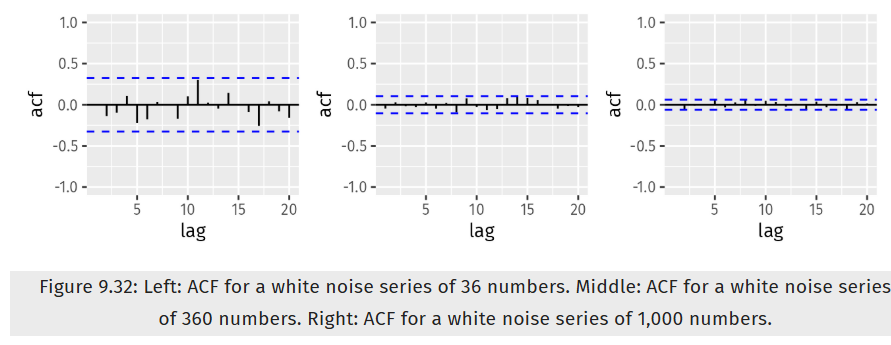
\includegraphics[keepaspectratio]{https://raw.githubusercontent.com/jhnboyy/CUNY_SPS_WORK/refs/heads/main/Spring2025/DATA624/Homework6/Figure932.png}}
\caption{Figure 9.32}
\end{figure}

\paragraph{a) Explain the differences among these figures. Do they all
indicate that the data are white
noise?}\label{a-explain-the-differences-among-these-figures.-do-they-all-indicate-that-the-data-are-white-noise}

In this figure there are several sub figures. It seems that the left
most figure contains white noise, as there doesn't seem to be any
discernible pattern in variances being plotted here. The middle image,
does not seem to be white noise, although its possible. There could be
somewhat of a pattern in this middle sub figure, while super subtle, the
pattern could to be similar to that of a sine wave with varying degrees
of strength. For this image, the strength of the sine-like pattern seems
to oscillate. That is it starts off small, gets a but stronger, and then
diminishes again. Lastly, the right-most sub figure seems to be white
noise. While there are portions of this sub figure that could be
somewhat of a pattern, overall it seems to be just noise. None of the
plotted values in these charts exceed the 95\% confidence interval
lines.

\paragraph{b) Why are the critical values at different distances from
the mean of zero? Why are the autocorrelations different in each figure
when they each refer to white
noise?}\label{b-why-are-the-critical-values-at-different-distances-from-the-mean-of-zero-why-are-the-autocorrelations-different-in-each-figure-when-they-each-refer-to-white-noise}

The critical values are at different distances from the mean of zero
because of the dataset they are plotted from. Going from left to right,
the dataset consisted of 36 random numbers 360 random numbers, and then
1000 random numbers. As the pool of random numbers got larger, the
confidence interval where 95\% of the data sits got more and more
narrow. With a smaller pool of numbers there is the potential for much
more variation in the numbers distribution, while larger random numbers
would follow more of a normal distribution pattern which would influence
the autocorrelation patterns. The autocorrelation patters are different
even though they each refer to white noise because the autocorrelation
is the numbers within a data set being compared to other numbers in the
same data set. So the variations in critical values and auto
correlations are going to be different for each grouping of random
numbers regardless of whether there is a pattern in the data or not.

\subsection{2) A classic example of a non-stationary series are stock
prices. Plot the daily closing prices for Amazon stock (contained in
gafa\_stock), along with the ACF and PACF. Explain how each plot shows
that the series is non-stationary and should be
differenced.}\label{a-classic-example-of-a-non-stationary-series-are-stock-prices.-plot-the-daily-closing-prices-for-amazon-stock-contained-in-gafa_stock-along-with-the-acf-and-pacf.-explain-how-each-plot-shows-that-the-series-is-non-stationary-and-should-be-differenced.}

\begin{Shaded}
\begin{Highlighting}[]
\CommentTok{\#table with just amazon}
\NormalTok{amazon }\OtherTok{\textless{}{-}}\NormalTok{ gafa\_stock }\SpecialCharTok{|\textgreater{}} \FunctionTok{filter}\NormalTok{(Symbol }\SpecialCharTok{==}\StringTok{\textquotesingle{}AMZN\textquotesingle{}}\NormalTok{)}\SpecialCharTok{|\textgreater{}} \FunctionTok{select}\NormalTok{(}\SpecialCharTok{{-}}\NormalTok{Open, }\SpecialCharTok{{-}}\NormalTok{High, }\SpecialCharTok{{-}}\NormalTok{Adj\_Close, }\SpecialCharTok{{-}}\NormalTok{Low, }\SpecialCharTok{{-}}\NormalTok{Volume)}
\FunctionTok{print}\NormalTok{(amazon }\SpecialCharTok{|\textgreater{}} \FunctionTok{autoplot}\NormalTok{())}
\end{Highlighting}
\end{Shaded}

\begin{verbatim}
## Plot variable not specified, automatically selected `.vars = Close`
\end{verbatim}

\pandocbounded{\includegraphics[keepaspectratio]{DATA624_Homework6_files/figure-latex/Exercise2-1.pdf}}

\begin{Shaded}
\begin{Highlighting}[]
\DocumentationTok{\#\# Here is the ACF and PACF plots for the raw non{-}differentiated or otherwise transformed data. }
\FunctionTok{print}\NormalTok{(amazon }\SpecialCharTok{|\textgreater{}} \FunctionTok{gg\_tsdisplay}\NormalTok{(Close,}\AttributeTok{plot\_type =}\StringTok{"partial"}\NormalTok{))}
\end{Highlighting}
\end{Shaded}

\begin{verbatim}
## Warning: Provided data has an irregular interval, results should be treated with caution. Computing ACF by observation.
## Provided data has an irregular interval, results should be treated with caution. Computing ACF by observation.
\end{verbatim}

\pandocbounded{\includegraphics[keepaspectratio]{DATA624_Homework6_files/figure-latex/Exercise2-2.pdf}}

\begin{Shaded}
\begin{Highlighting}[]
\DocumentationTok{\#\#\# After looking at these plots, firstly the data is not stationary. According to the first plot, there is a trend in the raw data that needs to be flattened out to have the same type of varying values for different sub time frames in this larger time frame. Additionally, when looking at the ACF chart all of the autocorrelation values start at 1 and slowly decrease just under 1. All of these values are very much so outside of the Confidence interval lines. This means there is a fairly consistent trend in the data, thus not stationary. Lastly, for the PACF chart there is a very large spike value in the beginning of the data,and 2 to 3 smaller spikes that are also outside the confidence interval band. This supports the non{-}stationary nature of the data.}


\DocumentationTok{\#\# No seasonality, but trends present in the close prices of the stock.}
\FunctionTok{print}\NormalTok{(amazon }\SpecialCharTok{|\textgreater{}} \FunctionTok{gg\_tsdisplay}\NormalTok{(}\FunctionTok{difference}\NormalTok{(}\FunctionTok{log}\NormalTok{(Close)),}\AttributeTok{plot\_type =}\StringTok{"partial"}\NormalTok{))}
\end{Highlighting}
\end{Shaded}

\begin{verbatim}
## Warning: Provided data has an irregular interval, results should be treated with caution. Computing ACF by observation.
## Provided data has an irregular interval, results should be treated with caution. Computing ACF by observation.
\end{verbatim}

\begin{verbatim}
## Warning: Removed 1 row containing missing values or values outside the scale range
## (`geom_line()`).
\end{verbatim}

\begin{verbatim}
## Warning: Removed 1 row containing missing values or values outside the scale range
## (`geom_point()`).
\end{verbatim}

\pandocbounded{\includegraphics[keepaspectratio]{DATA624_Homework6_files/figure-latex/Exercise2-3.pdf}}

\begin{Shaded}
\begin{Highlighting}[]
\CommentTok{\# Lastly, you can see here, with the logged and differentiated chart that the data is now stationary. There is no trend in the top chart, which now looks like white noise. The ACF and PACF charts both look much more reasonable with nearly all of the values being within the 95\% confidence interval range.}
\end{Highlighting}
\end{Shaded}

\subsection{3) For the following series, find an appropriate Box-Cox
transformation and order of differencing in order to obtain stationary
data.}\label{for-the-following-series-find-an-appropriate-box-cox-transformation-and-order-of-differencing-in-order-to-obtain-stationary-data.}

\paragraph{a) Turkish GDP from
global\_economy.}\label{a-turkish-gdp-from-global_economy.}

\begin{Shaded}
\begin{Highlighting}[]
\NormalTok{turkey\_economy }\OtherTok{\textless{}{-}}\NormalTok{ global\_economy }\SpecialCharTok{|\textgreater{}} \FunctionTok{filter}\NormalTok{(Country }\SpecialCharTok{==}\StringTok{\textquotesingle{}Turkey\textquotesingle{}}\NormalTok{)}

\FunctionTok{print}\NormalTok{(turkey\_economy}\SpecialCharTok{|\textgreater{}} \FunctionTok{autoplot}\NormalTok{())}
\end{Highlighting}
\end{Shaded}

\begin{verbatim}
## Plot variable not specified, automatically selected `.vars = GDP`
\end{verbatim}

\pandocbounded{\includegraphics[keepaspectratio]{DATA624_Homework6_files/figure-latex/Exercise3a-1.pdf}}

\begin{Shaded}
\begin{Highlighting}[]
\NormalTok{lambda }\OtherTok{\textless{}{-}}\NormalTok{ turkey\_economy }\SpecialCharTok{|\textgreater{}}
  \FunctionTok{features}\NormalTok{(GDP, }\AttributeTok{features =}\NormalTok{ guerrero) }\SpecialCharTok{|\textgreater{}}
  \FunctionTok{pull}\NormalTok{(lambda\_guerrero)}
\FunctionTok{print}\NormalTok{(lambda) }\DocumentationTok{\#\# 0.157 Close to a log transformation lambda}
\end{Highlighting}
\end{Shaded}

\begin{verbatim}
## [1] 0.1572187
\end{verbatim}

\begin{Shaded}
\begin{Highlighting}[]
\DocumentationTok{\#\# Box Cox Transform successful now to find the differentiation needs}
\FunctionTok{print}\NormalTok{(turkey\_economy }\SpecialCharTok{|\textgreater{}}  \FunctionTok{autoplot}\NormalTok{(}\FunctionTok{box\_cox}\NormalTok{(GDP, lambda)) }\SpecialCharTok{+}  \FunctionTok{labs}\NormalTok{(}\AttributeTok{y =} \StringTok{""}\NormalTok{,}\AttributeTok{title =}\NormalTok{ latex2exp}\SpecialCharTok{::}\FunctionTok{TeX}\NormalTok{(}\FunctionTok{paste0}\NormalTok{(}\StringTok{"BoxCox Transformed Turkey GDP"}\NormalTok{,}\FunctionTok{round}\NormalTok{(lambda,}\DecValTok{2}\NormalTok{)))))}
\end{Highlighting}
\end{Shaded}

\pandocbounded{\includegraphics[keepaspectratio]{DATA624_Homework6_files/figure-latex/Exercise3a-2.pdf}}

\begin{Shaded}
\begin{Highlighting}[]
\DocumentationTok{\#\# There is no seasonality in the data, just a general trend, performing one difference for the data. Seeing if second will be needed. Don\textquotesingle{}t think it is, as the data now seems stationary. The top plot is white noise, and the ACF and PACF plots are within the proper critical value bounds.}
\FunctionTok{print}\NormalTok{(turkey\_economy }\SpecialCharTok{|\textgreater{}} \FunctionTok{gg\_tsdisplay}\NormalTok{(}\FunctionTok{difference}\NormalTok{(}\FunctionTok{box\_cox}\NormalTok{(GDP, lambda)),}\AttributeTok{plot\_type =}\StringTok{"partial"}\NormalTok{, }\AttributeTok{lag=}\DecValTok{36}\NormalTok{))}
\end{Highlighting}
\end{Shaded}

\begin{verbatim}
## Warning: Removed 1 row containing missing values or values outside the scale range
## (`geom_line()`).
\end{verbatim}

\begin{verbatim}
## Warning: Removed 1 row containing missing values or values outside the scale range
## (`geom_point()`).
\end{verbatim}

\pandocbounded{\includegraphics[keepaspectratio]{DATA624_Homework6_files/figure-latex/Exercise3a-3.pdf}}

\paragraph{b) Accommodation takings in the state of Tasmania from
aus\_accommodation.}\label{b-accommodation-takings-in-the-state-of-tasmania-from-aus_accommodation.}

\begin{Shaded}
\begin{Highlighting}[]
\NormalTok{tasmania }\OtherTok{\textless{}{-}}\NormalTok{ aus\_accommodation }\SpecialCharTok{|\textgreater{}} \FunctionTok{filter}\NormalTok{(State }\SpecialCharTok{==} \StringTok{\textquotesingle{}Tasmania\textquotesingle{}}\NormalTok{)}
\DocumentationTok{\#\# Seasonality and trend in the data, needs to be smoothed out. }
\NormalTok{tasmania }\SpecialCharTok{|\textgreater{}} \FunctionTok{autoplot}\NormalTok{()}
\end{Highlighting}
\end{Shaded}

\begin{verbatim}
## Plot variable not specified, automatically selected `.vars = Takings`
\end{verbatim}

\pandocbounded{\includegraphics[keepaspectratio]{DATA624_Homework6_files/figure-latex/Exercise3b-1.pdf}}

\begin{Shaded}
\begin{Highlighting}[]
\DocumentationTok{\#\# Performing the Box Cox transformation }
\NormalTok{lambda }\OtherTok{\textless{}{-}}\NormalTok{ tasmania }\SpecialCharTok{|\textgreater{}}
  \FunctionTok{features}\NormalTok{(Takings, }\AttributeTok{features =}\NormalTok{ guerrero) }\SpecialCharTok{|\textgreater{}}
  \FunctionTok{pull}\NormalTok{(lambda\_guerrero)}
\FunctionTok{print}\NormalTok{(lambda) }\DocumentationTok{\#\# 0.0018 \#\# logging data is best.}
\end{Highlighting}
\end{Shaded}

\begin{verbatim}
## [1] 0.001819643
\end{verbatim}

\begin{Shaded}
\begin{Highlighting}[]
\DocumentationTok{\#\# Box Cox Transform successful now to find the differentiation needs}
\FunctionTok{print}\NormalTok{(tasmania }\SpecialCharTok{|\textgreater{}}  \FunctionTok{autoplot}\NormalTok{(}\FunctionTok{box\_cox}\NormalTok{(Takings, lambda)) }\SpecialCharTok{+}  \FunctionTok{labs}\NormalTok{(}\AttributeTok{y =} \StringTok{""}\NormalTok{,}\AttributeTok{title =}\NormalTok{ latex2exp}\SpecialCharTok{::}\FunctionTok{TeX}\NormalTok{(}\FunctionTok{paste0}\NormalTok{(}\StringTok{"BoxCox Transformed Takings for Tasmania"}\NormalTok{,}\FunctionTok{round}\NormalTok{(lambda,}\DecValTok{2}\NormalTok{)))))}
\end{Highlighting}
\end{Shaded}

\pandocbounded{\includegraphics[keepaspectratio]{DATA624_Homework6_files/figure-latex/Exercise3b-2.pdf}}

\begin{Shaded}
\begin{Highlighting}[]
\DocumentationTok{\#\# The seasonality is now constant(ish) and the trend looks better for differencing. In order to accommodate the seasonal nature of the data, we need to do a seasonal differencing. Doing a seasonal differencing of 4 because the data is quarterly.}

\FunctionTok{print}\NormalTok{(tasmania }\SpecialCharTok{|\textgreater{}} \FunctionTok{gg\_tsdisplay}\NormalTok{(}\FunctionTok{difference}\NormalTok{(Takings,}\DecValTok{4}\NormalTok{), }\AttributeTok{plot\_type=}\StringTok{\textquotesingle{}partial\textquotesingle{}}\NormalTok{, }\AttributeTok{lag=}\DecValTok{36}\NormalTok{))}
\end{Highlighting}
\end{Shaded}

\begin{verbatim}
## Warning: Removed 4 rows containing missing values or values outside the scale range
## (`geom_line()`).
\end{verbatim}

\begin{verbatim}
## Warning: Removed 4 rows containing missing values or values outside the scale range
## (`geom_point()`).
\end{verbatim}

\pandocbounded{\includegraphics[keepaspectratio]{DATA624_Homework6_files/figure-latex/Exercise3b-3.pdf}}

\begin{Shaded}
\begin{Highlighting}[]
\DocumentationTok{\#\# After looking at the data, it still does not seem completely stationary. The ACF has a trend, the PACF seems to have a slight one as well. There are also multiple values outside of the 95\% confidence interval boundaries, so there needs to be a second differencing here. }

\FunctionTok{print}\NormalTok{(tasmania }\SpecialCharTok{|\textgreater{}} \FunctionTok{gg\_tsdisplay}\NormalTok{(}\FunctionTok{difference}\NormalTok{(Takings,}\DecValTok{4}\NormalTok{)}\SpecialCharTok{|\textgreater{}} \FunctionTok{difference}\NormalTok{(), }\AttributeTok{plot\_type=}\StringTok{\textquotesingle{}partial\textquotesingle{}}\NormalTok{, }\AttributeTok{lag=}\DecValTok{36}\NormalTok{))}
\end{Highlighting}
\end{Shaded}

\begin{verbatim}
## Warning: Removed 5 rows containing missing values or values outside the scale range
## (`geom_line()`).
\end{verbatim}

\begin{verbatim}
## Warning: Removed 5 rows containing missing values or values outside the scale range
## (`geom_point()`).
\end{verbatim}

\pandocbounded{\includegraphics[keepaspectratio]{DATA624_Homework6_files/figure-latex/Exercise3b-4.pdf}}

\begin{Shaded}
\begin{Highlighting}[]
\DocumentationTok{\#\# The data now looks much more like white noise, and is probably stationary now. }
\end{Highlighting}
\end{Shaded}

\paragraph{c) Monthly sales from
souvenirs.}\label{c-monthly-sales-from-souvenirs.}

\begin{Shaded}
\begin{Highlighting}[]
\DocumentationTok{\#\# Taking a look at the data.}
\FunctionTok{print}\NormalTok{(souvenirs }\SpecialCharTok{|\textgreater{}} \FunctionTok{autoplot}\NormalTok{())}
\end{Highlighting}
\end{Shaded}

\begin{verbatim}
## Plot variable not specified, automatically selected `.vars = Sales`
\end{verbatim}

\pandocbounded{\includegraphics[keepaspectratio]{DATA624_Homework6_files/figure-latex/Exercise3c-1.pdf}}

\begin{Shaded}
\begin{Highlighting}[]
\DocumentationTok{\#\# There is both a trend and a seasonal pattern here. Using Box Cox to get proper transformation.}
\DocumentationTok{\#\# Performing the Box Cox transformation }
\NormalTok{lambda }\OtherTok{\textless{}{-}}\NormalTok{ souvenirs }\SpecialCharTok{|\textgreater{}}
  \FunctionTok{features}\NormalTok{(Sales, }\AttributeTok{features =}\NormalTok{ guerrero) }\SpecialCharTok{|\textgreater{}}
  \FunctionTok{pull}\NormalTok{(lambda\_guerrero)}
\FunctionTok{print}\NormalTok{(lambda) }\DocumentationTok{\#\# 0.00211 \#\# logging data is best.}
\end{Highlighting}
\end{Shaded}

\begin{verbatim}
## [1] 0.002118221
\end{verbatim}

\begin{Shaded}
\begin{Highlighting}[]
\DocumentationTok{\#\# Box Cox Transform successful now to find the differentiation needs}
\FunctionTok{print}\NormalTok{(souvenirs }\SpecialCharTok{|\textgreater{}}  \FunctionTok{autoplot}\NormalTok{(}\FunctionTok{box\_cox}\NormalTok{(Sales, lambda)) }\SpecialCharTok{+}  \FunctionTok{labs}\NormalTok{(}\AttributeTok{y =} \StringTok{""}\NormalTok{,}\AttributeTok{title =}\NormalTok{ latex2exp}\SpecialCharTok{::}\FunctionTok{TeX}\NormalTok{(}\FunctionTok{paste0}\NormalTok{(}\StringTok{"BoxCox Transformed Souvenirs Sales"}\NormalTok{,}\FunctionTok{round}\NormalTok{(lambda,}\DecValTok{2}\NormalTok{)))))}
\end{Highlighting}
\end{Shaded}

\pandocbounded{\includegraphics[keepaspectratio]{DATA624_Homework6_files/figure-latex/Exercise3c-2.pdf}}

\begin{Shaded}
\begin{Highlighting}[]
\DocumentationTok{\#\# eveled out a bit, now doing differencing, monthly for seasonal. (12)}
\FunctionTok{print}\NormalTok{(souvenirs }\SpecialCharTok{|\textgreater{}} \FunctionTok{gg\_tsdisplay}\NormalTok{(}\FunctionTok{difference}\NormalTok{(Sales,}\DecValTok{12}\NormalTok{), }\AttributeTok{plot\_type=}\StringTok{\textquotesingle{}partial\textquotesingle{}}\NormalTok{, }\AttributeTok{lag=}\DecValTok{36}\NormalTok{))}
\end{Highlighting}
\end{Shaded}

\begin{verbatim}
## Warning: Removed 12 rows containing missing values or values outside the scale range
## (`geom_line()`).
\end{verbatim}

\begin{verbatim}
## Warning: Removed 12 rows containing missing values or values outside the scale range
## (`geom_point()`).
\end{verbatim}

\pandocbounded{\includegraphics[keepaspectratio]{DATA624_Homework6_files/figure-latex/Exercise3c-3.pdf}}

\begin{Shaded}
\begin{Highlighting}[]
\DocumentationTok{\#\# Still needs more differencing for the trend. }
\FunctionTok{print}\NormalTok{(souvenirs }\SpecialCharTok{|\textgreater{}} \FunctionTok{gg\_tsdisplay}\NormalTok{(}\FunctionTok{difference}\NormalTok{(Sales,}\DecValTok{12}\NormalTok{) }\SpecialCharTok{|\textgreater{}} \FunctionTok{difference}\NormalTok{(), }\AttributeTok{plot\_type=}\StringTok{\textquotesingle{}partial\textquotesingle{}}\NormalTok{, }\AttributeTok{lag=}\DecValTok{36}\NormalTok{))}
\end{Highlighting}
\end{Shaded}

\begin{verbatim}
## Warning: Removed 13 rows containing missing values or values outside the scale range
## (`geom_line()`).
\end{verbatim}

\begin{verbatim}
## Warning: Removed 13 rows containing missing values or values outside the scale range
## (`geom_point()`).
\end{verbatim}

\pandocbounded{\includegraphics[keepaspectratio]{DATA624_Homework6_files/figure-latex/Exercise3c-4.pdf}}

\begin{Shaded}
\begin{Highlighting}[]
\DocumentationTok{\#\# Data finally looks stationary, however there are multiple instances of outliers for the ACF and the PACF. Similar for the top chart too. }
\end{Highlighting}
\end{Shaded}

\subsection{5) For your retail data (from Exercise 7 in Section 2.10),
find the appropriate order of differencing (after transformation if
necessary) to obtain stationary
data.}\label{for-your-retail-data-from-exercise-7-in-section-2.10-find-the-appropriate-order-of-differencing-after-transformation-if-necessary-to-obtain-stationary-data.}

\begin{Shaded}
\begin{Highlighting}[]
\DocumentationTok{\#\# CODE FROM CHAPTER 2 Number 7.}
\FunctionTok{set.seed}\NormalTok{(}\DecValTok{12345678}\NormalTok{)}
\NormalTok{myseries }\OtherTok{\textless{}{-}}\NormalTok{ aus\_retail }\SpecialCharTok{|\textgreater{}}
  \FunctionTok{filter}\NormalTok{(}\StringTok{\textasciigrave{}}\AttributeTok{Series ID}\StringTok{\textasciigrave{}} \SpecialCharTok{==} \FunctionTok{sample}\NormalTok{(aus\_retail}\SpecialCharTok{$}\StringTok{\textasciigrave{}}\AttributeTok{Series ID}\StringTok{\textasciigrave{}}\NormalTok{,}\DecValTok{1}\NormalTok{))}

\DocumentationTok{\#\# Taking a look at the data. There is both a trend and a seasonality in the data. The seasonality is getting more extreme over time, as it seems. These shifts arent constant.}
\NormalTok{myseries }\SpecialCharTok{|\textgreater{}} \FunctionTok{autoplot}\NormalTok{()}
\end{Highlighting}
\end{Shaded}

\begin{verbatim}
## Plot variable not specified, automatically selected `.vars = Turnover`
\end{verbatim}

\pandocbounded{\includegraphics[keepaspectratio]{DATA624_Homework6_files/figure-latex/exercise5-1.pdf}}

\begin{Shaded}
\begin{Highlighting}[]
\DocumentationTok{\#\#\# using Box Cox to get ideal transform value.}
\NormalTok{lambda }\OtherTok{\textless{}{-}}\NormalTok{ myseries }\SpecialCharTok{|\textgreater{}}
  \FunctionTok{features}\NormalTok{(Turnover, }\AttributeTok{features =}\NormalTok{ guerrero) }\SpecialCharTok{|\textgreater{}}
  \FunctionTok{pull}\NormalTok{(lambda\_guerrero)}
\FunctionTok{print}\NormalTok{(lambda) }\DocumentationTok{\#\# 0.083 \#\# inbetween sq root and now transform. }
\end{Highlighting}
\end{Shaded}

\begin{verbatim}
## [1] 0.08303631
\end{verbatim}

\begin{Shaded}
\begin{Highlighting}[]
\DocumentationTok{\#\# Looks better.}
\FunctionTok{print}\NormalTok{(myseries }\SpecialCharTok{|\textgreater{}}  \FunctionTok{autoplot}\NormalTok{(}\FunctionTok{box\_cox}\NormalTok{(Turnover, lambda)) }\SpecialCharTok{+}  \FunctionTok{labs}\NormalTok{(}\AttributeTok{y =} \StringTok{""}\NormalTok{,}\AttributeTok{title =}\NormalTok{ latex2exp}\SpecialCharTok{::}\FunctionTok{TeX}\NormalTok{(}\FunctionTok{paste0}\NormalTok{(}\StringTok{"BoxCox Transformed Retail Turnover"}\NormalTok{,}\FunctionTok{round}\NormalTok{(lambda,}\DecValTok{2}\NormalTok{)))))}
\end{Highlighting}
\end{Shaded}

\pandocbounded{\includegraphics[keepaspectratio]{DATA624_Homework6_files/figure-latex/exercise5-2.pdf}}

\begin{Shaded}
\begin{Highlighting}[]
\DocumentationTok{\#\# Starting Differencing. Will need 2 levels probably becuase of season and trend. Did with just one \& its not a enough, so jumping to 2}
\FunctionTok{print}\NormalTok{(myseries }\SpecialCharTok{|\textgreater{}} \FunctionTok{gg\_tsdisplay}\NormalTok{(}\FunctionTok{difference}\NormalTok{(Turnover,}\DecValTok{12}\NormalTok{) }\SpecialCharTok{|\textgreater{}} \FunctionTok{difference}\NormalTok{(), }\AttributeTok{plot\_type=}\StringTok{\textquotesingle{}partial\textquotesingle{}}\NormalTok{, }\AttributeTok{lag=}\DecValTok{36}\NormalTok{))}
\end{Highlighting}
\end{Shaded}

\begin{verbatim}
## Warning: Removed 13 rows containing missing values or values outside the scale range
## (`geom_line()`).
\end{verbatim}

\begin{verbatim}
## Warning: Removed 13 rows containing missing values or values outside the scale range
## (`geom_point()`).
\end{verbatim}

\pandocbounded{\includegraphics[keepaspectratio]{DATA624_Homework6_files/figure-latex/exercise5-3.pdf}}

\begin{Shaded}
\begin{Highlighting}[]
\DocumentationTok{\#\# After one transformation there was still a noticable trend in the data, after the second one it seems to be stationary / show white noise.}
\end{Highlighting}
\end{Shaded}

\subsection{6) Simulate and plot some data from simple ARIMA
models.}\label{simulate-and-plot-some-data-from-simple-arima-models.}

\paragraph{a)Use the following R code to generate data from an AR(1)
model with ϕ1 = 0.6 and σ2=1. The process starts with
y1=0.}\label{ause-the-following-r-code-to-generate-data-from-an-ar1-model-with-ux3d51-0.6-and-ux3c321.-the-process-starts-with-y10.}

\begin{Shaded}
\begin{Highlighting}[]
\FunctionTok{set.seed}\NormalTok{(}\DecValTok{12345678}\NormalTok{)}
\NormalTok{y }\OtherTok{\textless{}{-}} \FunctionTok{numeric}\NormalTok{(}\DecValTok{100}\NormalTok{)}
\NormalTok{e }\OtherTok{\textless{}{-}} \FunctionTok{rnorm}\NormalTok{(}\DecValTok{100}\NormalTok{)}
\ControlFlowTok{for}\NormalTok{(i }\ControlFlowTok{in} \DecValTok{2}\SpecialCharTok{:}\DecValTok{100}\NormalTok{)}
\NormalTok{  y[i] }\OtherTok{\textless{}{-}} \FloatTok{0.6}\SpecialCharTok{*}\NormalTok{y[i}\DecValTok{{-}1}\NormalTok{] }\SpecialCharTok{+}\NormalTok{ e[i]}
\NormalTok{sim }\OtherTok{\textless{}{-}} \FunctionTok{tsibble}\NormalTok{(}\AttributeTok{idx =} \FunctionTok{seq\_len}\NormalTok{(}\DecValTok{100}\NormalTok{), }\AttributeTok{y =}\NormalTok{ y, }\AttributeTok{index =}\NormalTok{ idx)}

\DocumentationTok{\#\# Looking at the random simulation. }
\FunctionTok{print}\NormalTok{(sim }\SpecialCharTok{|\textgreater{}} \FunctionTok{autoplot}\NormalTok{())}
\end{Highlighting}
\end{Shaded}

\begin{verbatim}
## Plot variable not specified, automatically selected `.vars = y`
\end{verbatim}

\pandocbounded{\includegraphics[keepaspectratio]{DATA624_Homework6_files/figure-latex/exercise6a_reference-1.pdf}}

\begin{Shaded}
\begin{Highlighting}[]
\DocumentationTok{\#\# No trend, just variations. No real cyclical / seasonal shifts, bit there is variation. Looking at the ACF and PACF to confirm AR(1). There is a gradual decay in the acf which is inline an ar(1) model, but there seems to be a pattern in the 20 {-} 30 range, but because of the small random sample size it is probably just chance. Then in the PACF there is one main spike at the beginning then only smaller values. }
\FunctionTok{print}\NormalTok{(sim }\SpecialCharTok{|\textgreater{}} \FunctionTok{gg\_tsdisplay}\NormalTok{(y, }\AttributeTok{plot\_type=}\StringTok{\textquotesingle{}partial\textquotesingle{}}\NormalTok{, }\AttributeTok{lag=}\DecValTok{36}\NormalTok{))}
\end{Highlighting}
\end{Shaded}

\pandocbounded{\includegraphics[keepaspectratio]{DATA624_Homework6_files/figure-latex/exercise6a_reference-2.pdf}}

\paragraph{b) Produce a time plot for the series. How does the plot
change as you change ϕ1
?}\label{b-produce-a-time-plot-for-the-series.-how-does-the-plot-change-as-you-change-ux3d51}

\begin{Shaded}
\begin{Highlighting}[]
\DocumentationTok{\#\# Firstly Doing autoplot of the original sim}
\FunctionTok{print}\NormalTok{(sim }\SpecialCharTok{|\textgreater{}} \FunctionTok{autoplot}\NormalTok{())}
\end{Highlighting}
\end{Shaded}

\begin{verbatim}
## Plot variable not specified, automatically selected `.vars = y`
\end{verbatim}

\pandocbounded{\includegraphics[keepaspectratio]{DATA624_Homework6_files/figure-latex/exercise6b-1.pdf}}

\begin{Shaded}
\begin{Highlighting}[]
\DocumentationTok{\#\#\# Running again with a different coefficients\#}
\NormalTok{y2 }\OtherTok{\textless{}{-}} \FunctionTok{numeric}\NormalTok{(}\DecValTok{100}\NormalTok{)}
\ControlFlowTok{for}\NormalTok{(i }\ControlFlowTok{in} \DecValTok{2}\SpecialCharTok{:}\DecValTok{100}\NormalTok{)}
\NormalTok{  y2[i] }\OtherTok{\textless{}{-}} \FloatTok{0.3}\SpecialCharTok{*}\NormalTok{y2[i}\DecValTok{{-}1}\NormalTok{] }\SpecialCharTok{+}\NormalTok{ e[i]}
\NormalTok{sim2 }\OtherTok{\textless{}{-}} \FunctionTok{tsibble}\NormalTok{(}\AttributeTok{idx =} \FunctionTok{seq\_len}\NormalTok{(}\DecValTok{100}\NormalTok{), }\AttributeTok{y =}\NormalTok{ y2, }\AttributeTok{index =}\NormalTok{ idx)}

\DocumentationTok{\#\# With 0.3}
\FunctionTok{print}\NormalTok{(sim2 }\SpecialCharTok{|\textgreater{}} \FunctionTok{autoplot}\NormalTok{())}
\end{Highlighting}
\end{Shaded}

\begin{verbatim}
## Plot variable not specified, automatically selected `.vars = y`
\end{verbatim}

\pandocbounded{\includegraphics[keepaspectratio]{DATA624_Homework6_files/figure-latex/exercise6b-2.pdf}}

\begin{Shaded}
\begin{Highlighting}[]
\DocumentationTok{\#\# Running agina with different coef.}
\NormalTok{y3 }\OtherTok{\textless{}{-}} \FunctionTok{numeric}\NormalTok{(}\DecValTok{100}\NormalTok{)}
\ControlFlowTok{for}\NormalTok{(i }\ControlFlowTok{in} \DecValTok{2}\SpecialCharTok{:}\DecValTok{100}\NormalTok{)}
\NormalTok{  y3[i] }\OtherTok{\textless{}{-}} \FloatTok{0.9}\SpecialCharTok{*}\NormalTok{y3[i}\DecValTok{{-}1}\NormalTok{] }\SpecialCharTok{+}\NormalTok{ e[i]}
\NormalTok{sim3 }\OtherTok{\textless{}{-}} \FunctionTok{tsibble}\NormalTok{(}\AttributeTok{idx =} \FunctionTok{seq\_len}\NormalTok{(}\DecValTok{100}\NormalTok{), }\AttributeTok{y =}\NormalTok{ y3, }\AttributeTok{index =}\NormalTok{ idx)}

\FunctionTok{print}\NormalTok{(sim3 }\SpecialCharTok{|\textgreater{}} \FunctionTok{autoplot}\NormalTok{())}
\end{Highlighting}
\end{Shaded}

\begin{verbatim}
## Plot variable not specified, automatically selected `.vars = y`
\end{verbatim}

\pandocbounded{\includegraphics[keepaspectratio]{DATA624_Homework6_files/figure-latex/exercise6b-3.pdf}}

\begin{Shaded}
\begin{Highlighting}[]
\DocumentationTok{\#\#\# Running again with a different coefficients\#}
\NormalTok{y2\_neg }\OtherTok{\textless{}{-}} \FunctionTok{numeric}\NormalTok{(}\DecValTok{100}\NormalTok{)}
\ControlFlowTok{for}\NormalTok{(i }\ControlFlowTok{in} \DecValTok{2}\SpecialCharTok{:}\DecValTok{100}\NormalTok{)}
\NormalTok{  y2\_neg[i] }\OtherTok{\textless{}{-}} \SpecialCharTok{{-}}\FloatTok{0.3}\SpecialCharTok{*}\NormalTok{y2\_neg[i}\DecValTok{{-}1}\NormalTok{] }\SpecialCharTok{+}\NormalTok{ e[i]}
\NormalTok{sim2\_neg }\OtherTok{\textless{}{-}} \FunctionTok{tsibble}\NormalTok{(}\AttributeTok{idx =} \FunctionTok{seq\_len}\NormalTok{(}\DecValTok{100}\NormalTok{), }\AttributeTok{y =}\NormalTok{ y2\_neg, }\AttributeTok{index =}\NormalTok{ idx)}

\DocumentationTok{\#\# With {-}0.3}
\FunctionTok{print}\NormalTok{(sim2\_neg }\SpecialCharTok{|\textgreater{}} \FunctionTok{autoplot}\NormalTok{())}
\end{Highlighting}
\end{Shaded}

\begin{verbatim}
## Plot variable not specified, automatically selected `.vars = y`
\end{verbatim}

\pandocbounded{\includegraphics[keepaspectratio]{DATA624_Homework6_files/figure-latex/exercise6b-4.pdf}}

\begin{Shaded}
\begin{Highlighting}[]
\DocumentationTok{\#\# Running again with a different coefficients\#}
\NormalTok{y\_neg }\OtherTok{\textless{}{-}} \FunctionTok{numeric}\NormalTok{(}\DecValTok{100}\NormalTok{)}
\ControlFlowTok{for}\NormalTok{(i }\ControlFlowTok{in} \DecValTok{2}\SpecialCharTok{:}\DecValTok{100}\NormalTok{)}
\NormalTok{  y\_neg[i] }\OtherTok{\textless{}{-}} \SpecialCharTok{{-}}\FloatTok{0.6}\SpecialCharTok{*}\NormalTok{y\_neg[i}\DecValTok{{-}1}\NormalTok{] }\SpecialCharTok{+}\NormalTok{ e[i]}
\NormalTok{sim\_neg }\OtherTok{\textless{}{-}} \FunctionTok{tsibble}\NormalTok{(}\AttributeTok{idx =} \FunctionTok{seq\_len}\NormalTok{(}\DecValTok{100}\NormalTok{), }\AttributeTok{y =}\NormalTok{ y\_neg, }\AttributeTok{index =}\NormalTok{ idx)}

\FunctionTok{print}\NormalTok{(sim\_neg }\SpecialCharTok{|\textgreater{}} \FunctionTok{autoplot}\NormalTok{())}
\end{Highlighting}
\end{Shaded}

\begin{verbatim}
## Plot variable not specified, automatically selected `.vars = y`
\end{verbatim}

\pandocbounded{\includegraphics[keepaspectratio]{DATA624_Homework6_files/figure-latex/exercise6b-5.pdf}}

\begin{Shaded}
\begin{Highlighting}[]
\DocumentationTok{\#\# Running agina with different coef.}
\NormalTok{y3\_neg }\OtherTok{\textless{}{-}} \FunctionTok{numeric}\NormalTok{(}\DecValTok{100}\NormalTok{)}
\ControlFlowTok{for}\NormalTok{(i }\ControlFlowTok{in} \DecValTok{2}\SpecialCharTok{:}\DecValTok{100}\NormalTok{)}
\NormalTok{  y3\_neg[i] }\OtherTok{\textless{}{-}} \SpecialCharTok{{-}}\FloatTok{0.9}\SpecialCharTok{*}\NormalTok{y3\_neg[i}\DecValTok{{-}1}\NormalTok{] }\SpecialCharTok{+}\NormalTok{ e[i]}
\NormalTok{sim3\_neg }\OtherTok{\textless{}{-}} \FunctionTok{tsibble}\NormalTok{(}\AttributeTok{idx =} \FunctionTok{seq\_len}\NormalTok{(}\DecValTok{100}\NormalTok{), }\AttributeTok{y =}\NormalTok{ y3\_neg, }\AttributeTok{index =}\NormalTok{ idx)}

\FunctionTok{print}\NormalTok{(sim3\_neg }\SpecialCharTok{|\textgreater{}} \FunctionTok{autoplot}\NormalTok{())}
\end{Highlighting}
\end{Shaded}

\begin{verbatim}
## Plot variable not specified, automatically selected `.vars = y`
\end{verbatim}

\pandocbounded{\includegraphics[keepaspectratio]{DATA624_Homework6_files/figure-latex/exercise6b-6.pdf}}

\begin{Shaded}
\begin{Highlighting}[]
\DocumentationTok{\#\# The lower the coefficient (when positive) the variation seems to be a bit more intense, when the positive coefficients get larger the variation in the data seems to be slightly less exaggerated. When dealing with negative coefficients, the closer to negative one that the coefficient is the more frequency and exaggerated nature of the variations in the data increases.}
\end{Highlighting}
\end{Shaded}

\paragraph{c) Write your own code to generate data from an MA(1) model
with θ1=0.6 and
σ2=1.}\label{c-write-your-own-code-to-generate-data-from-an-ma1-model-with-ux3b810.6-and-ux3c321.}

\begin{Shaded}
\begin{Highlighting}[]
\NormalTok{y }\OtherTok{\textless{}{-}} \FunctionTok{numeric}\NormalTok{(}\DecValTok{100}\NormalTok{)}
\NormalTok{e }\OtherTok{\textless{}{-}} \FunctionTok{rnorm}\NormalTok{(}\DecValTok{100}\NormalTok{, }\AttributeTok{sd=}\DecValTok{1}\NormalTok{)}
\ControlFlowTok{for}\NormalTok{(i }\ControlFlowTok{in} \DecValTok{2}\SpecialCharTok{:}\DecValTok{100}\NormalTok{)}
\NormalTok{  y[i] }\OtherTok{\textless{}{-}}\NormalTok{ e[i]}\SpecialCharTok{+}\FloatTok{0.6}\SpecialCharTok{*}\NormalTok{e[i}\DecValTok{{-}1}\NormalTok{]}
\NormalTok{sim\_ma }\OtherTok{\textless{}{-}} \FunctionTok{tsibble}\NormalTok{(}\AttributeTok{idx =} \FunctionTok{seq\_len}\NormalTok{(}\DecValTok{100}\NormalTok{), }\AttributeTok{y =}\NormalTok{ y, }\AttributeTok{index =}\NormalTok{ idx)}

\NormalTok{sim\_ma }\SpecialCharTok{|\textgreater{}} \FunctionTok{autoplot}\NormalTok{()}
\end{Highlighting}
\end{Shaded}

\begin{verbatim}
## Plot variable not specified, automatically selected `.vars = y`
\end{verbatim}

\pandocbounded{\includegraphics[keepaspectratio]{DATA624_Homework6_files/figure-latex/exercise6c-1.pdf}}

\paragraph{d) Produce a time plot for the series. How does the plot
change as you change
θ1?}\label{d-produce-a-time-plot-for-the-series.-how-does-the-plot-change-as-you-change-ux3b81}

\begin{Shaded}
\begin{Highlighting}[]
\CommentTok{\# Doing {-}0.3, {-}0.6, {-}0.9, 0.3, 0.6, 0.9}
\CommentTok{\#Original}
\FunctionTok{print}\NormalTok{(sim\_ma }\SpecialCharTok{|\textgreater{}} \FunctionTok{autoplot}\NormalTok{())}
\end{Highlighting}
\end{Shaded}

\begin{verbatim}
## Plot variable not specified, automatically selected `.vars = y`
\end{verbatim}

\pandocbounded{\includegraphics[keepaspectratio]{DATA624_Homework6_files/figure-latex/exercise6d-1.pdf}}

\begin{Shaded}
\begin{Highlighting}[]
\DocumentationTok{\#\#\# Running again with a different coefficients}
\NormalTok{yma\_2 }\OtherTok{\textless{}{-}} \FunctionTok{numeric}\NormalTok{(}\DecValTok{100}\NormalTok{)}
\ControlFlowTok{for}\NormalTok{(i }\ControlFlowTok{in} \DecValTok{2}\SpecialCharTok{:}\DecValTok{100}\NormalTok{)}
\NormalTok{  yma\_2[i] }\OtherTok{\textless{}{-}}\NormalTok{ e[i]}\SpecialCharTok{+}\FloatTok{0.3}\SpecialCharTok{*}\NormalTok{e[i}\DecValTok{{-}1}\NormalTok{]}
\NormalTok{simma\_2 }\OtherTok{\textless{}{-}} \FunctionTok{tsibble}\NormalTok{(}\AttributeTok{idx =} \FunctionTok{seq\_len}\NormalTok{(}\DecValTok{100}\NormalTok{), }\AttributeTok{y =}\NormalTok{ yma\_2, }\AttributeTok{index =}\NormalTok{ idx)}

\DocumentationTok{\#\# With 0.3}
\FunctionTok{print}\NormalTok{(simma\_2 }\SpecialCharTok{|\textgreater{}} \FunctionTok{autoplot}\NormalTok{())}
\end{Highlighting}
\end{Shaded}

\begin{verbatim}
## Plot variable not specified, automatically selected `.vars = y`
\end{verbatim}

\pandocbounded{\includegraphics[keepaspectratio]{DATA624_Homework6_files/figure-latex/exercise6d-2.pdf}}

\begin{Shaded}
\begin{Highlighting}[]
\CommentTok{\# With 0.9}
\NormalTok{yma\_3 }\OtherTok{\textless{}{-}} \FunctionTok{numeric}\NormalTok{(}\DecValTok{100}\NormalTok{)}
\ControlFlowTok{for}\NormalTok{(i }\ControlFlowTok{in} \DecValTok{2}\SpecialCharTok{:}\DecValTok{100}\NormalTok{)}
\NormalTok{  yma\_3[i] }\OtherTok{\textless{}{-}}\NormalTok{ e[i]}\SpecialCharTok{+}\FloatTok{0.9}\SpecialCharTok{*}\NormalTok{e[i}\DecValTok{{-}1}\NormalTok{]}
\NormalTok{simma\_3 }\OtherTok{\textless{}{-}} \FunctionTok{tsibble}\NormalTok{(}\AttributeTok{idx =} \FunctionTok{seq\_len}\NormalTok{(}\DecValTok{100}\NormalTok{), }\AttributeTok{y =}\NormalTok{ yma\_3, }\AttributeTok{index =}\NormalTok{ idx)}

\FunctionTok{print}\NormalTok{(simma\_3 }\SpecialCharTok{|\textgreater{}} \FunctionTok{autoplot}\NormalTok{())}
\end{Highlighting}
\end{Shaded}

\begin{verbatim}
## Plot variable not specified, automatically selected `.vars = y`
\end{verbatim}

\pandocbounded{\includegraphics[keepaspectratio]{DATA624_Homework6_files/figure-latex/exercise6d-3.pdf}}

\begin{Shaded}
\begin{Highlighting}[]
\DocumentationTok{\#\#\# With {-}0.3}
\NormalTok{yma\_2\_neg }\OtherTok{\textless{}{-}} \FunctionTok{numeric}\NormalTok{(}\DecValTok{100}\NormalTok{)}
\ControlFlowTok{for}\NormalTok{(i }\ControlFlowTok{in} \DecValTok{2}\SpecialCharTok{:}\DecValTok{100}\NormalTok{)}
\NormalTok{  yma\_2\_neg[i] }\OtherTok{\textless{}{-}}\NormalTok{ e[i]}\SpecialCharTok{{-}}\FloatTok{0.3}\SpecialCharTok{*}\NormalTok{e[i}\DecValTok{{-}1}\NormalTok{]}
\NormalTok{simma2\_neg }\OtherTok{\textless{}{-}} \FunctionTok{tsibble}\NormalTok{(}\AttributeTok{idx =} \FunctionTok{seq\_len}\NormalTok{(}\DecValTok{100}\NormalTok{), }\AttributeTok{y =}\NormalTok{ yma\_2\_neg, }\AttributeTok{index =}\NormalTok{ idx)}

\FunctionTok{print}\NormalTok{(simma2\_neg }\SpecialCharTok{|\textgreater{}} \FunctionTok{autoplot}\NormalTok{())}
\end{Highlighting}
\end{Shaded}

\begin{verbatim}
## Plot variable not specified, automatically selected `.vars = y`
\end{verbatim}

\pandocbounded{\includegraphics[keepaspectratio]{DATA624_Homework6_files/figure-latex/exercise6d-4.pdf}}

\begin{Shaded}
\begin{Highlighting}[]
\DocumentationTok{\#\# {-}0.6}
\NormalTok{yma\_neg }\OtherTok{\textless{}{-}} \FunctionTok{numeric}\NormalTok{(}\DecValTok{100}\NormalTok{)}
\ControlFlowTok{for}\NormalTok{(i }\ControlFlowTok{in} \DecValTok{2}\SpecialCharTok{:}\DecValTok{100}\NormalTok{)}
\NormalTok{  yma\_neg[i] }\OtherTok{\textless{}{-}}\NormalTok{ e[i]}\SpecialCharTok{{-}}\FloatTok{0.6}\SpecialCharTok{*}\NormalTok{e[i}\DecValTok{{-}1}\NormalTok{]}
\NormalTok{simma\_neg }\OtherTok{\textless{}{-}} \FunctionTok{tsibble}\NormalTok{(}\AttributeTok{idx =} \FunctionTok{seq\_len}\NormalTok{(}\DecValTok{100}\NormalTok{), }\AttributeTok{y =}\NormalTok{ yma\_neg, }\AttributeTok{index =}\NormalTok{ idx)}

\FunctionTok{print}\NormalTok{(simma\_neg }\SpecialCharTok{|\textgreater{}} \FunctionTok{autoplot}\NormalTok{())}
\end{Highlighting}
\end{Shaded}

\begin{verbatim}
## Plot variable not specified, automatically selected `.vars = y`
\end{verbatim}

\pandocbounded{\includegraphics[keepaspectratio]{DATA624_Homework6_files/figure-latex/exercise6d-5.pdf}}

\begin{Shaded}
\begin{Highlighting}[]
\DocumentationTok{\#\# With {-}0.9.}
\NormalTok{yma3\_neg }\OtherTok{\textless{}{-}} \FunctionTok{numeric}\NormalTok{(}\DecValTok{100}\NormalTok{)}
\ControlFlowTok{for}\NormalTok{(i }\ControlFlowTok{in} \DecValTok{2}\SpecialCharTok{:}\DecValTok{100}\NormalTok{)}
\NormalTok{  yma3\_neg[i] }\OtherTok{\textless{}{-}}\NormalTok{ e[i]}\SpecialCharTok{{-}}\FloatTok{0.9}\SpecialCharTok{*}\NormalTok{e[i}\DecValTok{{-}1}\NormalTok{]}
\NormalTok{simma3\_neg }\OtherTok{\textless{}{-}} \FunctionTok{tsibble}\NormalTok{(}\AttributeTok{idx =} \FunctionTok{seq\_len}\NormalTok{(}\DecValTok{100}\NormalTok{), }\AttributeTok{y =}\NormalTok{ yma3\_neg, }\AttributeTok{index =}\NormalTok{ idx)}

\FunctionTok{print}\NormalTok{(simma3\_neg }\SpecialCharTok{|\textgreater{}} \FunctionTok{autoplot}\NormalTok{())}
\end{Highlighting}
\end{Shaded}

\begin{verbatim}
## Plot variable not specified, automatically selected `.vars = y`
\end{verbatim}

\pandocbounded{\includegraphics[keepaspectratio]{DATA624_Homework6_files/figure-latex/exercise6d-6.pdf}}

\begin{Shaded}
\begin{Highlighting}[]
\CommentTok{\# There really isn\textquotesingle{}t much variation with the shift in moving average model coefficients, there arent any big changes in the data. }
\end{Highlighting}
\end{Shaded}

\paragraph{e) Generate data from an ARMA(1,1) model with ϕ1=0.6, θ1=0.6
and
σ2=1.}\label{e-generate-data-from-an-arma11-model-with-ux3d510.6-ux3b810.6-and-ux3c321.}

\begin{Shaded}
\begin{Highlighting}[]
\CommentTok{\#Generating new ARMA model.}
\FunctionTok{set.seed}\NormalTok{(}\DecValTok{123}\NormalTok{)}
\NormalTok{y\_arma }\OtherTok{\textless{}{-}} \FunctionTok{numeric}\NormalTok{(}\DecValTok{100}\NormalTok{)}
\NormalTok{e\_arma }\OtherTok{\textless{}{-}} \FunctionTok{rnorm}\NormalTok{(}\DecValTok{100}\NormalTok{, }\AttributeTok{sd=}\DecValTok{1}\NormalTok{) }\CommentTok{\#σ2=1}
\ControlFlowTok{for}\NormalTok{(i }\ControlFlowTok{in} \DecValTok{2}\SpecialCharTok{:}\DecValTok{100}\NormalTok{)}
\NormalTok{  y\_arma[i] }\OtherTok{\textless{}{-}} \FloatTok{0.6}\SpecialCharTok{*}\NormalTok{y\_arma[i}\DecValTok{{-}1}\NormalTok{] }\SpecialCharTok{+}\NormalTok{ e\_arma[i] }\SpecialCharTok{+} \FloatTok{0.6}\SpecialCharTok{*}\NormalTok{e\_arma[i}\DecValTok{{-}1}\NormalTok{]}
\NormalTok{sim\_arma }\OtherTok{\textless{}{-}} \FunctionTok{tsibble}\NormalTok{(}\AttributeTok{idx =} \FunctionTok{seq\_len}\NormalTok{(}\DecValTok{100}\NormalTok{), }\AttributeTok{y =}\NormalTok{ y\_arma, }\AttributeTok{index =}\NormalTok{ idx)}
\end{Highlighting}
\end{Shaded}

\paragraph{f) Generate data from an AR(2) model with ϕ1=−0.8, ϕ2=0.3 and
σ2=1. (Note that these parameters will give a non-stationary
series.)}\label{f-generate-data-from-an-ar2-model-with-ux3d510.8-ux3d520.3-and-ux3c321.-note-that-these-parameters-will-give-a-non-stationary-series.}

\begin{Shaded}
\begin{Highlighting}[]
\DocumentationTok{\#\# Applying the coefficients into a formula like above. }
\NormalTok{y\_ar2 }\OtherTok{\textless{}{-}} \FunctionTok{numeric}\NormalTok{(}\DecValTok{100}\NormalTok{)}
\NormalTok{e\_ar2 }\OtherTok{\textless{}{-}} \FunctionTok{rnorm}\NormalTok{(}\DecValTok{100}\NormalTok{, }\AttributeTok{sd=}\DecValTok{1}\NormalTok{)}
\ControlFlowTok{for}\NormalTok{(i }\ControlFlowTok{in} \DecValTok{3}\SpecialCharTok{:}\DecValTok{100}\NormalTok{)}
\NormalTok{  y\_ar2[i] }\OtherTok{\textless{}{-}} \FloatTok{0.8}\SpecialCharTok{*}\NormalTok{y\_ar2[i}\DecValTok{{-}1}\NormalTok{] }\SpecialCharTok{+} \FloatTok{0.3}\SpecialCharTok{*}\NormalTok{y\_ar2[i}\DecValTok{{-}2}\NormalTok{] }\SpecialCharTok{+}\NormalTok{ e\_ar2[i]}
\NormalTok{sim\_ar2 }\OtherTok{\textless{}{-}} \FunctionTok{tsibble}\NormalTok{(}\AttributeTok{idx =} \FunctionTok{seq\_len}\NormalTok{(}\DecValTok{100}\NormalTok{), }\AttributeTok{y =}\NormalTok{ y\_ar2, }\AttributeTok{index =}\NormalTok{ idx)}
\end{Highlighting}
\end{Shaded}

\paragraph{g) Graph the latter two series and compare
them.}\label{g-graph-the-latter-two-series-and-compare-them.}

\begin{Shaded}
\begin{Highlighting}[]
\CommentTok{\#plotting  ARMA(1,1)}
\FunctionTok{print}\NormalTok{(sim\_arma }\SpecialCharTok{|\textgreater{}} \FunctionTok{autoplot}\NormalTok{())}
\end{Highlighting}
\end{Shaded}

\begin{verbatim}
## Plot variable not specified, automatically selected `.vars = y`
\end{verbatim}

\pandocbounded{\includegraphics[keepaspectratio]{DATA624_Homework6_files/figure-latex/exercise6g-1.pdf}}

\begin{Shaded}
\begin{Highlighting}[]
\CommentTok{\#plotting AR(2)}
\FunctionTok{print}\NormalTok{(sim\_ar2}\SpecialCharTok{|\textgreater{}} \FunctionTok{autoplot}\NormalTok{())}
\end{Highlighting}
\end{Shaded}

\begin{verbatim}
## Plot variable not specified, automatically selected `.vars = y`
\end{verbatim}

\pandocbounded{\includegraphics[keepaspectratio]{DATA624_Homework6_files/figure-latex/exercise6g-2.pdf}}

\begin{Shaded}
\begin{Highlighting}[]
\DocumentationTok{\#\#\# When looking at the plots of both of these charts, it is obvious that the first ARMA(1,1) model does not really have a trend but simply has variations in the data. There doesnt seem to be a discernable pattern there. However, in the second of the two, the AS(2) model, there is an obvious, almost exponential trend downwards. }
\end{Highlighting}
\end{Shaded}

\subsection{7) Consider aus\_airpassengers, the total number of
passengers (in millions) from Australian air carriers for the period
1970-2011.}\label{consider-aus_airpassengers-the-total-number-of-passengers-in-millions-from-australian-air-carriers-for-the-period-1970-2011.}

\paragraph{a) Use ARIMA() to find an appropriate ARIMA model. What model
was selected. Check that the residuals look like white noise. Plot
forecasts for the next 10
periods.}\label{a-use-arima-to-find-an-appropriate-arima-model.-what-model-was-selected.-check-that-the-residuals-look-like-white-noise.-plot-forecasts-for-the-next-10-periods.}

\begin{Shaded}
\begin{Highlighting}[]
\CommentTok{\# plotting first {-} No real seasonality here, just upward trend over time. }
\FunctionTok{print}\NormalTok{(aus\_airpassengers }\SpecialCharTok{|\textgreater{}} \FunctionTok{autoplot}\NormalTok{())}
\end{Highlighting}
\end{Shaded}

\begin{verbatim}
## Plot variable not specified, automatically selected `.vars = Passengers`
\end{verbatim}

\pandocbounded{\includegraphics[keepaspectratio]{DATA624_Homework6_files/figure-latex/exercise7a-1.pdf}}

\begin{Shaded}
\begin{Highlighting}[]
\DocumentationTok{\#\# Using built in ARIMA}
\NormalTok{fit1 }\OtherTok{\textless{}{-}}\NormalTok{ aus\_airpassengers }\SpecialCharTok{|\textgreater{}}
  \FunctionTok{model}\NormalTok{(}\FunctionTok{ARIMA}\NormalTok{(Passengers))}

\DocumentationTok{\#\# Printing the decision of the model selector function}
\FunctionTok{print}\NormalTok{(}\FunctionTok{report}\NormalTok{(fit1))}
\end{Highlighting}
\end{Shaded}

\begin{verbatim}
## Series: Passengers 
## Model: ARIMA(0,2,1) 
## 
## Coefficients:
##           ma1
##       -0.8963
## s.e.   0.0594
## 
## sigma^2 estimated as 4.308:  log likelihood=-97.02
## AIC=198.04   AICc=198.32   BIC=201.65
## # A mable: 1 x 1
##   `ARIMA(Passengers)`
##               <model>
## 1      <ARIMA(0,2,1)>
\end{verbatim}

\begin{Shaded}
\begin{Highlighting}[]
\DocumentationTok{\#\#\#\textless{}OUTPUT\textgreater{}}
\DocumentationTok{\#\#\#Series: Passengers }
\DocumentationTok{\#\#\#Model: ARIMA(0,2,1) }

\DocumentationTok{\#\#\#Coefficients:}
\DocumentationTok{\#\#\#          ma1}
\DocumentationTok{\#\#\#      {-}0.8963}
\DocumentationTok{\#\#\# s.e.   0.0594}

\DocumentationTok{\#\#\#sigma\^{}2 estimated as 4.308:  log likelihood={-}97.02}
\DocumentationTok{\#\#\#AIC=198.04   AICc=198.32   BIC=201.65}


\DocumentationTok{\#\# The arima function found that an ARIMA(0,2,1) model was the best fit for the data. This means that no AR modeling techniques were used in the model, and only Moving Averaging was used. There were also 2 levels of differencing applied. The moving average coefficient that was a best fit to the data was {-}0.8963 with a standard error of 0.059. The standard deviation was about 4.3.}

\DocumentationTok{\#\# looking at residuals}
\FunctionTok{print}\NormalTok{(}\FunctionTok{gg\_tsresiduals}\NormalTok{(fit1))}
\end{Highlighting}
\end{Shaded}

\pandocbounded{\includegraphics[keepaspectratio]{DATA624_Homework6_files/figure-latex/exercise7a-2.pdf}}

\begin{Shaded}
\begin{Highlighting}[]
\DocumentationTok{\#\# The residuals do look like white noise. The acf as no patterns to speak of and the counts are basially normally distributed. }

\DocumentationTok{\#\# Predicting the next ten years with the model}
\FunctionTok{print}\NormalTok{(fit1 }\SpecialCharTok{|\textgreater{}} \FunctionTok{forecast}\NormalTok{(}\AttributeTok{h=}\DecValTok{10}\NormalTok{) }\SpecialCharTok{|\textgreater{}} \FunctionTok{autoplot}\NormalTok{(aus\_airpassengers) }\SpecialCharTok{+} \FunctionTok{labs}\NormalTok{(}\AttributeTok{y =} \StringTok{"Passengers"}\NormalTok{, }\AttributeTok{title =} \StringTok{"Australian Air Carrier Passengers"}\NormalTok{))}
\end{Highlighting}
\end{Shaded}

\pandocbounded{\includegraphics[keepaspectratio]{DATA624_Homework6_files/figure-latex/exercise7a-3.pdf}}

\paragraph{b) Write the model in terms of the backshift
operator.}\label{b-write-the-model-in-terms-of-the-backshift-operator.}

\begin{Shaded}
\begin{Highlighting}[]
\CommentTok{\#ARIMA(0,2,1)}
\CommentTok{\#p=0 \#\# No AR}
\CommentTok{\#d=2 \#\# number of differences}
\CommentTok{\#q=1 \#\# MA one t diff. }

\DocumentationTok{\#\# Replacing with backshift filling from textbook}
\CommentTok{\#(1−B)\^{}2y[t] = {-}0.8963(B)ε[t]}
\end{Highlighting}
\end{Shaded}

\subsubsection{c) Plot forecasts from an ARIMA(0,1,0) model with drift
and compare these to part
a.}\label{c-plot-forecasts-from-an-arima010-model-with-drift-and-compare-these-to-part-a.}

\begin{Shaded}
\begin{Highlighting}[]
\DocumentationTok{\#\# Using built in ARIMA}
\NormalTok{fit2 }\OtherTok{\textless{}{-}}\NormalTok{ aus\_airpassengers }\SpecialCharTok{|\textgreater{}}  \FunctionTok{model}\NormalTok{(}\FunctionTok{ARIMA}\NormalTok{(Passengers }\SpecialCharTok{\textasciitilde{}} \DecValTok{1}\SpecialCharTok{+} \FunctionTok{pdq}\NormalTok{(}\DecValTok{0}\NormalTok{,}\DecValTok{1}\NormalTok{,}\DecValTok{0}\NormalTok{) )) }\CommentTok{\#}

\DocumentationTok{\#\# Printing the decision of the model selector function}
\FunctionTok{print}\NormalTok{(}\FunctionTok{report}\NormalTok{(fit2))}
\end{Highlighting}
\end{Shaded}

\begin{verbatim}
## Series: Passengers 
## Model: ARIMA(0,1,0) w/ drift 
## 
## Coefficients:
##       constant
##         1.4191
## s.e.    0.3014
## 
## sigma^2 estimated as 4.271:  log likelihood=-98.16
## AIC=200.31   AICc=200.59   BIC=203.97
## # A mable: 1 x 1
##   `ARIMA(Passengers ~ 1 + pdq(0, 1, 0))`
##                                  <model>
## 1                <ARIMA(0,1,0) w/ drift>
\end{verbatim}

\begin{Shaded}
\begin{Highlighting}[]
\CommentTok{\#Coefficients:}
\CommentTok{\#          ar1      ar2     ma1     ma2  constant}
\CommentTok{\#      {-}0.5518  {-}0.7327  0.5895  1.0000    3.2216}
\CommentTok{\#s.e.   0.1684   0.1224  0.0916  0.1008    0.7224}

\CommentTok{\#sigma\^{}2 estimated as 4.031:  log likelihood={-}96.23}
\CommentTok{\#AIC=204.46   AICc=206.61   BIC=215.43}

\CommentTok{\#Residuals}
\FunctionTok{print}\NormalTok{(}\FunctionTok{gg\_tsresiduals}\NormalTok{(fit2))}
\end{Highlighting}
\end{Shaded}

\pandocbounded{\includegraphics[keepaspectratio]{DATA624_Homework6_files/figure-latex/exercise7c-1.pdf}}

\begin{Shaded}
\begin{Highlighting}[]
\DocumentationTok{\#\# When comparing to part a, the residual counts seem a little more normally distributed. The ACF chart has less negative values, but still is white noise. Similarly, The top chart seems to be pretty similar as well. }

\DocumentationTok{\#\# Predicting the next ten years with the model}
\FunctionTok{print}\NormalTok{(fit2 }\SpecialCharTok{|\textgreater{}} \FunctionTok{forecast}\NormalTok{(}\AttributeTok{h=}\DecValTok{10}\NormalTok{) }\SpecialCharTok{|\textgreater{}} \FunctionTok{autoplot}\NormalTok{(aus\_airpassengers) }\SpecialCharTok{+} \FunctionTok{labs}\NormalTok{(}\AttributeTok{y =} \StringTok{"Passengers"}\NormalTok{, }\AttributeTok{title =} \StringTok{"Australian Air Carrier Passengers"}\NormalTok{))}
\end{Highlighting}
\end{Shaded}

\pandocbounded{\includegraphics[keepaspectratio]{DATA624_Homework6_files/figure-latex/exercise7c-2.pdf}}

\begin{Shaded}
\begin{Highlighting}[]
\DocumentationTok{\#\# When compared to part a, the forecast is slightly less upwards with this forecast being a bit more blunted in terms of predicted increase in passengers over the next ten years.}
\end{Highlighting}
\end{Shaded}

\paragraph{d) Plot forecasts from an ARIMA(2,1,2) model with drift and
compare these to parts a and c.~Remove the constant and see what
happens.}\label{d-plot-forecasts-from-an-arima212-model-with-drift-and-compare-these-to-parts-a-and-c.-remove-the-constant-and-see-what-happens.}

\begin{Shaded}
\begin{Highlighting}[]
\NormalTok{fit3 }\OtherTok{\textless{}{-}}\NormalTok{ aus\_airpassengers }\SpecialCharTok{|\textgreater{}}   \FunctionTok{model}\NormalTok{(}\FunctionTok{ARIMA}\NormalTok{(Passengers }\SpecialCharTok{\textasciitilde{}} \DecValTok{1}\SpecialCharTok{+} \FunctionTok{pdq}\NormalTok{(}\DecValTok{2}\NormalTok{,}\DecValTok{1}\NormalTok{,}\DecValTok{2}\NormalTok{)))}

\FunctionTok{print}\NormalTok{(}\FunctionTok{report}\NormalTok{(fit3))}
\end{Highlighting}
\end{Shaded}

\begin{verbatim}
## Series: Passengers 
## Model: ARIMA(2,1,2) w/ drift 
## 
## Coefficients:
##           ar1      ar2     ma1     ma2  constant
##       -0.5518  -0.7327  0.5895  1.0000    3.2216
## s.e.   0.1684   0.1224  0.0916  0.1008    0.7224
## 
## sigma^2 estimated as 4.031:  log likelihood=-96.23
## AIC=204.46   AICc=206.61   BIC=215.43
## # A mable: 1 x 1
##   `ARIMA(Passengers ~ 1 + pdq(2, 1, 2))`
##                                  <model>
## 1                <ARIMA(2,1,2) w/ drift>
\end{verbatim}

\begin{Shaded}
\begin{Highlighting}[]
\CommentTok{\#Coefficients:}
\CommentTok{\#          ar1      ar2     ma1     ma2  constant}
\CommentTok{\#      {-}0.5518  {-}0.7327  0.5895  1.0000    3.2216}
\CommentTok{\#s.e.   0.1684   0.1224  0.0916  0.1008    0.7224}

\CommentTok{\#sigma\^{}2 estimated as 4.031:  log likelihood={-}96.23}
\CommentTok{\#AIC=204.46   AICc=206.61   BIC=215.43}

\FunctionTok{print}\NormalTok{(}\FunctionTok{gg\_tsresiduals}\NormalTok{(fit3))}
\end{Highlighting}
\end{Shaded}

\pandocbounded{\includegraphics[keepaspectratio]{DATA624_Homework6_files/figure-latex/exercise7d-1.pdf}}

\begin{Shaded}
\begin{Highlighting}[]
\CommentTok{\# The residual distribution is less normal than those in part a and c, That is the main difference i see in the residuals plot. }

\CommentTok{\#Forecast}
\FunctionTok{print}\NormalTok{(fit3 }\SpecialCharTok{|\textgreater{}} \FunctionTok{forecast}\NormalTok{(}\AttributeTok{h=}\DecValTok{10}\NormalTok{) }\SpecialCharTok{|\textgreater{}} \FunctionTok{autoplot}\NormalTok{(aus\_airpassengers) }\SpecialCharTok{+} \FunctionTok{labs}\NormalTok{(}\AttributeTok{y =} \StringTok{"Passengers"}\NormalTok{, }\AttributeTok{title =} \StringTok{"Australian Air Carrier Passengers"}\NormalTok{))}
\end{Highlighting}
\end{Shaded}

\pandocbounded{\includegraphics[keepaspectratio]{DATA624_Homework6_files/figure-latex/exercise7d-2.pdf}}

\begin{Shaded}
\begin{Highlighting}[]
\CommentTok{\# The forecast with this model is less straight. The link itself is more "wiggled" which means it is more susceptible to fluctuations in the data.}


\DocumentationTok{\#\#\#\# Removign the Constant to see any shift}

\NormalTok{fit3\_nc }\OtherTok{\textless{}{-}}\NormalTok{ aus\_airpassengers }\SpecialCharTok{|\textgreater{}}   \FunctionTok{model}\NormalTok{(}\FunctionTok{ARIMA}\NormalTok{(Passengers }\SpecialCharTok{\textasciitilde{}} \FunctionTok{pdq}\NormalTok{(}\DecValTok{2}\NormalTok{,}\DecValTok{1}\NormalTok{,}\DecValTok{2}\NormalTok{)))}
\end{Highlighting}
\end{Shaded}

\begin{verbatim}
## Warning: It looks like you're trying to fully specify your ARIMA model but have not said if a constant should be included.
## You can include a constant using `ARIMA(y~1)` to the formula or exclude it by adding `ARIMA(y~0)`.
\end{verbatim}

\begin{verbatim}
## Warning: 1 error encountered for ARIMA(Passengers ~ pdq(2, 1, 2))
## [1] Could not find an appropriate ARIMA model.
## This is likely because automatic selection does not select models with characteristic roots that may be numerically unstable.
## For more details, refer to https://otexts.com/fpp3/arima-r.html#plotting-the-characteristic-roots
\end{verbatim}

\begin{Shaded}
\begin{Highlighting}[]
\DocumentationTok{\#\# When i remove the constant from the model i get the following warning along with a null model. }

\CommentTok{\#Warning: It looks like you\textquotesingle{}re trying to fully specify your ARIMA model but have not said if a constant should be included.}
\CommentTok{\#You can include a constant using \textasciigrave{}ARIMA(y\textasciitilde{}1)\textasciigrave{} to the formula or exclude it by adding \textasciigrave{}ARIMA(y\textasciitilde{}0)\textasciigrave{}.Warning: 1 error encountered for ARIMA(Passengers \textasciitilde{} pdq(2, 1, 2))}
\CommentTok{\#[1] Could not find an appropriate ARIMA model.}
\end{Highlighting}
\end{Shaded}

\paragraph{e) Plot forecasts from an ARIMA(0,2,1) model with a constant.
What
happens?}\label{e-plot-forecasts-from-an-arima021-model-with-a-constant.-what-happens}

\begin{Shaded}
\begin{Highlighting}[]
\NormalTok{fit4 }\OtherTok{\textless{}{-}}\NormalTok{ aus\_airpassengers }\SpecialCharTok{|\textgreater{}}  \FunctionTok{model}\NormalTok{(}\FunctionTok{ARIMA}\NormalTok{(Passengers }\SpecialCharTok{\textasciitilde{}} \DecValTok{1}\SpecialCharTok{+} \FunctionTok{pdq}\NormalTok{(}\DecValTok{0}\NormalTok{,}\DecValTok{2}\NormalTok{,}\DecValTok{1}\NormalTok{) )) }\CommentTok{\#}
\end{Highlighting}
\end{Shaded}

\begin{verbatim}
## Warning: Model specification induces a quadratic or higher order polynomial trend. 
## This is generally discouraged, consider removing the constant or reducing the number of differences.
\end{verbatim}

\begin{Shaded}
\begin{Highlighting}[]
\DocumentationTok{\#\# pritnign report }
\FunctionTok{print}\NormalTok{(}\FunctionTok{report}\NormalTok{(fit4))}
\end{Highlighting}
\end{Shaded}

\begin{verbatim}
## Series: Passengers 
## Model: ARIMA(0,2,1) w/ poly 
## 
## Coefficients:
##           ma1  constant
##       -1.0000    0.0571
## s.e.   0.0585    0.0213
## 
## sigma^2 estimated as 3.855:  log likelihood=-95.1
## AIC=196.21   AICc=196.79   BIC=201.63
## # A mable: 1 x 1
##   `ARIMA(Passengers ~ 1 + pdq(0, 2, 1))`
##                                  <model>
## 1                 <ARIMA(0,2,1) w/ poly>
\end{verbatim}

\begin{Shaded}
\begin{Highlighting}[]
\CommentTok{\#Output}
\CommentTok{\#Coefficients:}
\CommentTok{\#          ma1  constant}
\CommentTok{\#      {-}1.0000    0.0571}
\CommentTok{\#s.e.   0.0585    0.0213}

\CommentTok{\#sigma\^{}2 estimated as 3.855:  log likelihood={-}95.1}
\CommentTok{\#AIC=196.21   AICc=196.79   BIC=201.63}


\DocumentationTok{\#\# Residuals}
\FunctionTok{print}\NormalTok{(}\FunctionTok{gg\_tsresiduals}\NormalTok{(fit4))}
\end{Highlighting}
\end{Shaded}

\pandocbounded{\includegraphics[keepaspectratio]{DATA624_Homework6_files/figure-latex/exercise7e-1.pdf}}

\begin{Shaded}
\begin{Highlighting}[]
\CommentTok{\# The redsidual distribtuion has multiple outliers which may be problematic. The other charts seem to be ok though. }

\DocumentationTok{\#\# Forecast }
\FunctionTok{print}\NormalTok{(fit4 }\SpecialCharTok{|\textgreater{}} \FunctionTok{forecast}\NormalTok{(}\AttributeTok{h=}\DecValTok{10}\NormalTok{) }\SpecialCharTok{|\textgreater{}} \FunctionTok{autoplot}\NormalTok{(aus\_airpassengers) }\SpecialCharTok{+} \FunctionTok{labs}\NormalTok{(}\AttributeTok{y =} \StringTok{"Passengers"}\NormalTok{, }\AttributeTok{title =} \StringTok{"Australian Air Carrier Passengers"}\NormalTok{))}
\end{Highlighting}
\end{Shaded}

\pandocbounded{\includegraphics[keepaspectratio]{DATA624_Homework6_files/figure-latex/exercise7e-2.pdf}}

\begin{Shaded}
\begin{Highlighting}[]
\DocumentationTok{\#\#The forecast for this model increases more than the previous ones. Particularly, the confidence intervals go up to nearly 120 on the y axis, where in the other models it stays lower. The confidence interval bands are also narrower, which means the slope of the overall prediction is much more steep than the other models. }
\end{Highlighting}
\end{Shaded}

\subsection{8) For the United States GDP series (from
global\_economy):}\label{for-the-united-states-gdp-series-from-global_economy}

\paragraph{a) if necessary, find a suitable Box-Cox transformation for
the
data;}\label{a-if-necessary-find-a-suitable-box-cox-transformation-for-the-data}

\begin{Shaded}
\begin{Highlighting}[]
\CommentTok{\#print(unique(global\_economy$Country))}
\NormalTok{us\_gdp }\OtherTok{\textless{}{-}}\NormalTok{ global\_economy}\SpecialCharTok{|\textgreater{}} \FunctionTok{filter}\NormalTok{(Country }\SpecialCharTok{==} \StringTok{"United States"}\NormalTok{)}

\DocumentationTok{\#\# Viewing the data}
\NormalTok{us\_gdp }\SpecialCharTok{|\textgreater{}} \FunctionTok{autoplot}\NormalTok{()}
\end{Highlighting}
\end{Shaded}

\begin{verbatim}
## Plot variable not specified, automatically selected `.vars = GDP`
\end{verbatim}

\pandocbounded{\includegraphics[keepaspectratio]{DATA624_Homework6_files/figure-latex/exercise8a-1.pdf}}

\begin{Shaded}
\begin{Highlighting}[]
\DocumentationTok{\#\# Mainly a trend upwards, no seasonality or cyclical anything. }

\DocumentationTok{\#\#\# using Box Cox to get ideal transform value.}
\NormalTok{lambda }\OtherTok{\textless{}{-}}\NormalTok{ us\_gdp }\SpecialCharTok{|\textgreater{}}
  \FunctionTok{features}\NormalTok{(GDP, }\AttributeTok{features =}\NormalTok{ guerrero) }\SpecialCharTok{|\textgreater{}}
  \FunctionTok{pull}\NormalTok{(lambda\_guerrero)}
\FunctionTok{print}\NormalTok{(lambda) }\DocumentationTok{\#\# 0.2619}
\end{Highlighting}
\end{Shaded}

\begin{verbatim}
## [1] 0.2819443
\end{verbatim}

\begin{Shaded}
\begin{Highlighting}[]
\DocumentationTok{\#\# Looks better.}
\FunctionTok{print}\NormalTok{(us\_gdp }\SpecialCharTok{|\textgreater{}}  \FunctionTok{autoplot}\NormalTok{(}\FunctionTok{box\_cox}\NormalTok{(GDP, lambda)) }\SpecialCharTok{+}  \FunctionTok{labs}\NormalTok{(}\AttributeTok{y =} \StringTok{""}\NormalTok{,}\AttributeTok{title =}\NormalTok{ latex2exp}\SpecialCharTok{::}\FunctionTok{TeX}\NormalTok{(}\FunctionTok{paste0}\NormalTok{(}\StringTok{"BoxCox Transformed Retail Turnover "}\NormalTok{,}\FunctionTok{round}\NormalTok{(lambda,}\DecValTok{2}\NormalTok{)))))}
\end{Highlighting}
\end{Shaded}

\pandocbounded{\includegraphics[keepaspectratio]{DATA624_Homework6_files/figure-latex/exercise8a-2.pdf}}

\paragraph{b) fit a suitable ARIMA model to the transformed data using
ARIMA();}\label{b-fit-a-suitable-arima-model-to-the-transformed-data-using-arima}

\begin{Shaded}
\begin{Highlighting}[]
\CommentTok{\#Getting the ideal model using ARIMA}
\NormalTok{fit\_usgdp }\OtherTok{\textless{}{-}}\NormalTok{ us\_gdp }\SpecialCharTok{|\textgreater{}}  \FunctionTok{model}\NormalTok{(}\FunctionTok{ARIMA}\NormalTok{(}\FunctionTok{box\_cox}\NormalTok{(GDP, lambda)))}
\DocumentationTok{\#\# Model chosen was ARIMA (1,1,0)}
\FunctionTok{report}\NormalTok{(fit\_usgdp)}
\end{Highlighting}
\end{Shaded}

\begin{verbatim}
## Series: GDP 
## Model: ARIMA(1,1,0) w/ drift 
## Transformation: box_cox(GDP, lambda) 
## 
## Coefficients:
##          ar1  constant
##       0.4586  118.1822
## s.e.  0.1198    9.5047
## 
## sigma^2 estimated as 5479:  log likelihood=-325.32
## AIC=656.65   AICc=657.1   BIC=662.78
\end{verbatim}

\begin{Shaded}
\begin{Highlighting}[]
\CommentTok{\#\textless{}OUTPUT\textgreater{}}
\CommentTok{\#Coefficients:}
\CommentTok{\#         ar1  constant}
\CommentTok{\#      0.4586  118.1822}
\CommentTok{\#s.e.  0.1198    9.5047}

\CommentTok{\#sigma\^{}2 estimated as 5479:  log likelihood={-}325.32}
\CommentTok{\#AIC=656.65   AICc=657.1   BIC=662.78}
\end{Highlighting}
\end{Shaded}

\paragraph{c) try some other plausible models by experimenting with the
orders
chosen;}\label{c-try-some-other-plausible-models-by-experimenting-with-the-orders-chosen}

\begin{Shaded}
\begin{Highlighting}[]
\DocumentationTok{\#\# Going to do ARIMA(2,1,0); so one differencing and 2 look back wieghtings}
\NormalTok{fit\_usgdp2 }\OtherTok{\textless{}{-}}\NormalTok{ us\_gdp }\SpecialCharTok{|\textgreater{}}  \FunctionTok{model}\NormalTok{(}\FunctionTok{ARIMA}\NormalTok{(}\FunctionTok{box\_cox}\NormalTok{(GDP, lambda) }\SpecialCharTok{\textasciitilde{}} \FunctionTok{pdq}\NormalTok{(}\DecValTok{2}\NormalTok{,}\DecValTok{1}\NormalTok{,}\DecValTok{0}\NormalTok{)))}
\FunctionTok{report}\NormalTok{(fit\_usgdp2)}
\end{Highlighting}
\end{Shaded}

\begin{verbatim}
## Series: GDP 
## Model: ARIMA(2,1,0) w/ drift 
## Transformation: box_cox(GDP, lambda) 
## 
## Coefficients:
##          ar1     ar2  constant
##       0.4554  0.0071  117.2907
## s.e.  0.1341  0.1352    9.5225
## 
## sigma^2 estimated as 5580:  log likelihood=-325.32
## AIC=658.64   AICc=659.41   BIC=666.82
\end{verbatim}

\begin{Shaded}
\begin{Highlighting}[]
\DocumentationTok{\#\# \textless{}OUTPUT\textgreater{}}
\CommentTok{\#Coefficients:}
\CommentTok{\#         ar1     ar2  constant}
\CommentTok{\#      0.4554  0.0071  117.2907}
\CommentTok{\#s.e.  0.1341  0.1352    9.5225}

\CommentTok{\#sigma\^{}2 estimated as 5580:  log likelihood={-}325.32}
\CommentTok{\#AIC=658.64   AICc=659.41   BIC=666.82}
\end{Highlighting}
\end{Shaded}

\paragraph{d) choose what you think is the best model and check the
residual
diagnostics;}\label{d-choose-what-you-think-is-the-best-model-and-check-the-residual-diagnostics}

\begin{Shaded}
\begin{Highlighting}[]
\DocumentationTok{\#\# Choosing the first model as the numbers when looking at the AIC, the BIC, and the AICc, are the most ideal. The second model i tried not that much different, but got worse results with these benchmarks. }


\CommentTok{\#Looking at residuals}
\FunctionTok{gg\_tsresiduals}\NormalTok{(fit\_usgdp)}
\end{Highlighting}
\end{Shaded}

\pandocbounded{\includegraphics[keepaspectratio]{DATA624_Homework6_files/figure-latex/exercise8d-1.pdf}}

\begin{Shaded}
\begin{Highlighting}[]
\DocumentationTok{\#\# These plots seem to check out, the data is stationary and white noise. There are no discernible patterns in the top chart, or the acf chart. The residual count chart does seem to have a slight patterns, but could just be chance. The residuals are mostly normal looking.}
\end{Highlighting}
\end{Shaded}

\paragraph{e) produce forecasts of your fitted model. Do the forecasts
look
reasonable?}\label{e-produce-forecasts-of-your-fitted-model.-do-the-forecasts-look-reasonable}

\begin{Shaded}
\begin{Highlighting}[]
\CommentTok{\# Forcasting with the chosen models. }
\FunctionTok{print}\NormalTok{(fit\_usgdp }\SpecialCharTok{|\textgreater{}} \FunctionTok{forecast}\NormalTok{(}\AttributeTok{h=}\DecValTok{10}\NormalTok{) }\SpecialCharTok{|\textgreater{}} \FunctionTok{autoplot}\NormalTok{(us\_gdp) }\SpecialCharTok{+} \FunctionTok{labs}\NormalTok{(}\AttributeTok{y =} \StringTok{"GDP"}\NormalTok{, }\AttributeTok{title =} \StringTok{"United States GDP Forcast (ARIMA)"}\NormalTok{))}
\end{Highlighting}
\end{Shaded}

\pandocbounded{\includegraphics[keepaspectratio]{DATA624_Homework6_files/figure-latex/exercise8e-1.pdf}}

\begin{Shaded}
\begin{Highlighting}[]
\DocumentationTok{\#\# Yes, the forecast does seem reasonable. It very much appears to continue the trend already existant in the data. }
\end{Highlighting}
\end{Shaded}

\paragraph{f) compare the results with what you would obtain using ETS()
(with no
transformation).}\label{f-compare-the-results-with-what-you-would-obtain-using-ets-with-no-transformation.}

\begin{Shaded}
\begin{Highlighting}[]
\NormalTok{us\_gdp\_ets }\OtherTok{\textless{}{-}}\NormalTok{ us\_gdp }\SpecialCharTok{|\textgreater{}}  \FunctionTok{model}\NormalTok{(}\FunctionTok{ETS}\NormalTok{(GDP))}

\FunctionTok{print}\NormalTok{(}\FunctionTok{report}\NormalTok{(us\_gdp\_ets))}
\end{Highlighting}
\end{Shaded}

\begin{verbatim}
## Series: GDP 
## Model: ETS(M,A,N) 
##   Smoothing parameters:
##     alpha = 0.9990876 
##     beta  = 0.5011949 
## 
##   Initial states:
##          l[0]        b[0]
##  448093333334 64917355687
## 
##   sigma^2:  7e-04
## 
##      AIC     AICc      BIC 
## 3190.787 3191.941 3201.089 
## # A mable: 1 x 2
## # Key:     Country [1]
##   Country         `ETS(GDP)`
##   <fct>              <model>
## 1 United States <ETS(M,A,N)>
\end{verbatim}

\begin{Shaded}
\begin{Highlighting}[]
\FunctionTok{print}\NormalTok{(us\_gdp\_ets }\SpecialCharTok{|\textgreater{}} \FunctionTok{forecast}\NormalTok{(}\AttributeTok{h=}\DecValTok{10}\NormalTok{) }\SpecialCharTok{|\textgreater{}} \FunctionTok{autoplot}\NormalTok{(us\_gdp) }\SpecialCharTok{+} \FunctionTok{labs}\NormalTok{(}\AttributeTok{y =} \StringTok{"GDP"}\NormalTok{, }\AttributeTok{title =} \StringTok{"United States GDP Forcast (ETS)"}\NormalTok{))}
\end{Highlighting}
\end{Shaded}

\pandocbounded{\includegraphics[keepaspectratio]{DATA624_Homework6_files/figure-latex/exercise8f-1.pdf}}

\begin{Shaded}
\begin{Highlighting}[]
\CommentTok{\# The results from the ETS model versus the ARIMA model are different. The ETS forecast does not trend as upward as the ARIMA model does. In addition to that, the confidence intervals for the ARIMA model was much more narrow., while the ETS model seemed much more uncertain as to what was possible. }
\end{Highlighting}
\end{Shaded}


\end{document}
